\documentclass[mathserif,serif]{beamer}
\usepackage{pdfpages} 
\usepackage{graphics}
\usepackage{amsmath,amssymb,amsfonts,textcomp,setspace,graphicx,lipsum,hanging,url}
\setbeamercolor{frametitle}{fg=black}
\begin{document}
  \begin{frame}
    \frametitle{\centerline{NFL Go For It!}\\ \centerline{The 4th Down Decision}}
    %Frame 1
\begin{figure}
\begin{center}
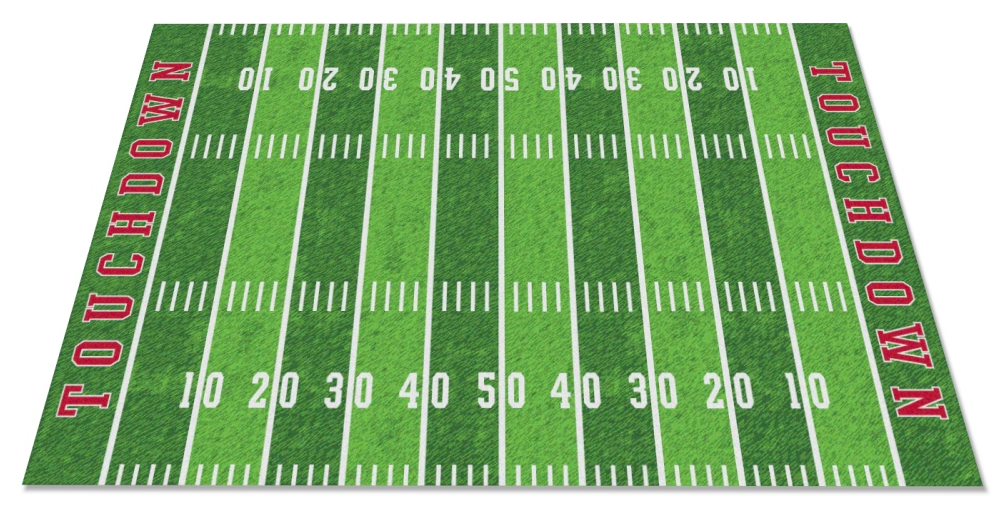
\includegraphics[width=1\textwidth]{FootballField.png}
\end{center}
\end{figure}
\begin{center}
by Mike Ghirardo and Thomas McCann
\end{center}
  \end{frame}
\begin{frame}
 \frametitle{\centerline{NFL Go For It!}}
In football there are many decisions a team needs to make in order to win the game. In this project we focus on those that need to be made on 4th down plays. Following are the three decisions to be made on the fourth down. \\
\begin{enumerate}[1.]
\item 
Punt
\item
Kick a field goal
\item
Go for a first down
\end{enumerate}
\end{frame}
\begin{frame}
 \frametitle{\centerline{NFL Go For It!}}
We attempt to determine which choice should be made under certain conditions. The following are the conditions which we take into account in determining the best action.
\begin{enumerate}[1.]
\item
Offensive and defensive rank of the offensive team
\item
Offensive and defensive rank of the defensive team
\item
The number of yards to convert a first down
\item
The field position
\end{enumerate}
With this information from the data we were able to estimate the expected points scored given each of the three decisions.\\
Finally, with this information a decision can be made.
\end{frame}
  \begin{frame}
    \frametitle{\centerline{NFL Go For It!}}
    %Frame 2
\centerline{The Data}
The data that we have chosen to attempt to answer this research question is NFL play-by-play data for seasons 2002 - 2012. The play-by-play data includes a game ID, which quarter, which down, which teams, a play description, and the number of points scored. A lot of of data cleaning and manipulation was required to successfully analyze the data and even more work may be required to get more accurate predictions.  From the data we ranked the teams according to their defense and offense to minimize any team specific effects that is inherent in the data. 
  \end{frame}
 \begin{frame}
    \frametitle{\centerline{NFL Go For It!}}
\centerline{Determining the Decision}
Let $Points_{o}$ and $Points_{d}$ be the number of points the offensive and defensive team will score respectively. Let $Punt$, $Field Goal$, and $Go For It$ be the events that the offensive team punts, attempts a field goal and goes for the 1st down given they are on their fourth down respectively. Let $S_{f}$ and $S_{g}$ be the events that the offensive team successfully scores a field goal and successfully converts a first down respectively. Then let
{\footnotesize
\begin{gather*}
P = E[Points_{o} | Punt] \\
G = E[Points_{o}|Go For It] = E[Points_{o}| S_{g}]P(S_{g}) - E[Points_{d}|S_{g}^c]P(S_{g}^c)\\
F = E[Points_{o}|Field Goal] = E[Points_{o}| S_{f}]P(S_{f}) - E[Points_{d}|S_{f}^c]P(S_{f}^c)\\
\end{gather*}
}%
Then Decision $= argmax\{P, G, F\}$.
  \end{frame}
  \begin{frame}
    \frametitle{\centerline{NFL Go For It!}}
\begin{figure}
\begin{center}
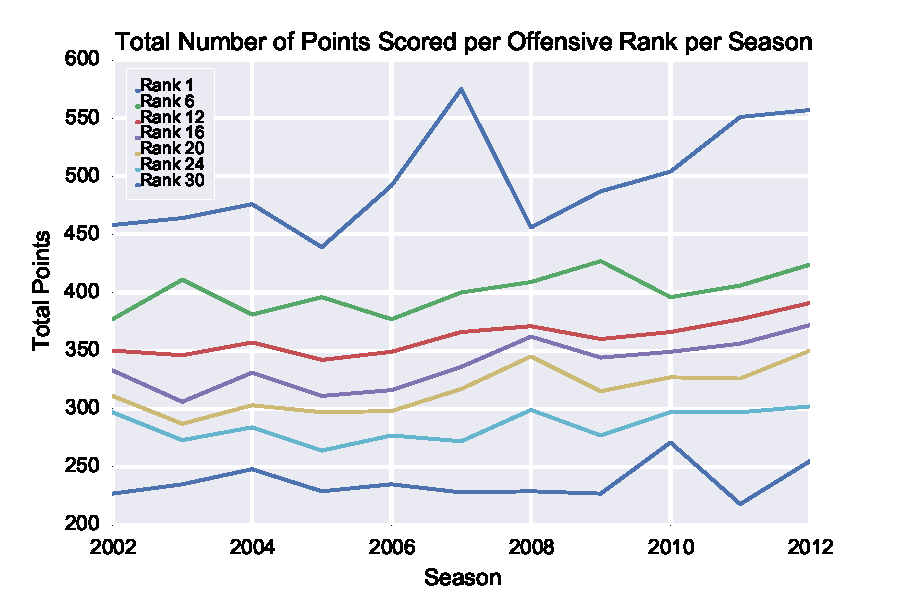
\includegraphics[width=1\textwidth]{OffRankperSeason.pdf}
\end{center}
\end{figure}
  \end{frame}
  \begin{frame}
    \frametitle{\centerline{NFL Go For It!}}
\begin{figure}
\begin{center}
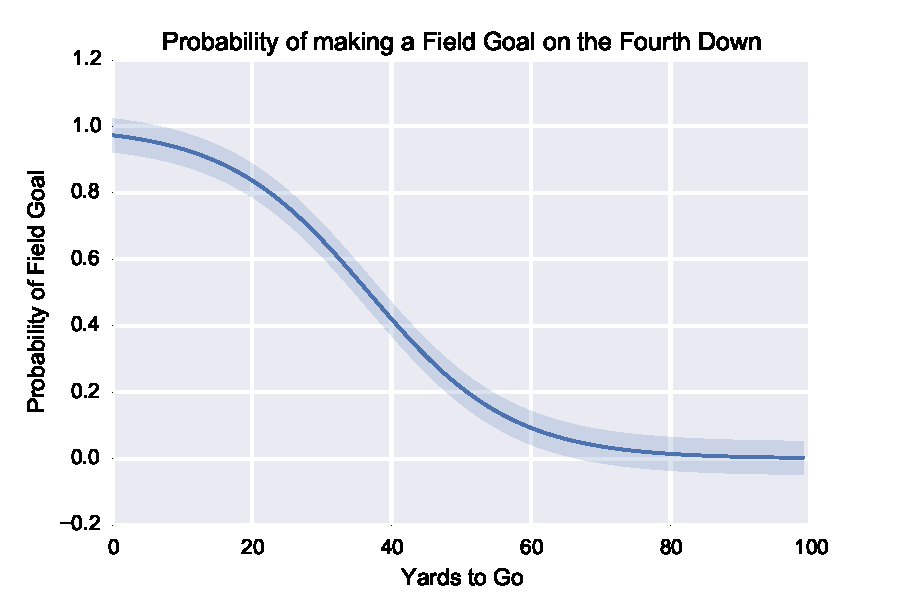
\includegraphics[width=1\textwidth]{fieldgoalprob.pdf}
\end{center}
\end{figure}
  \end{frame}
  \begin{frame}
    \frametitle{\centerline{NFL Go For It!}}
\begin{figure}
\begin{center}
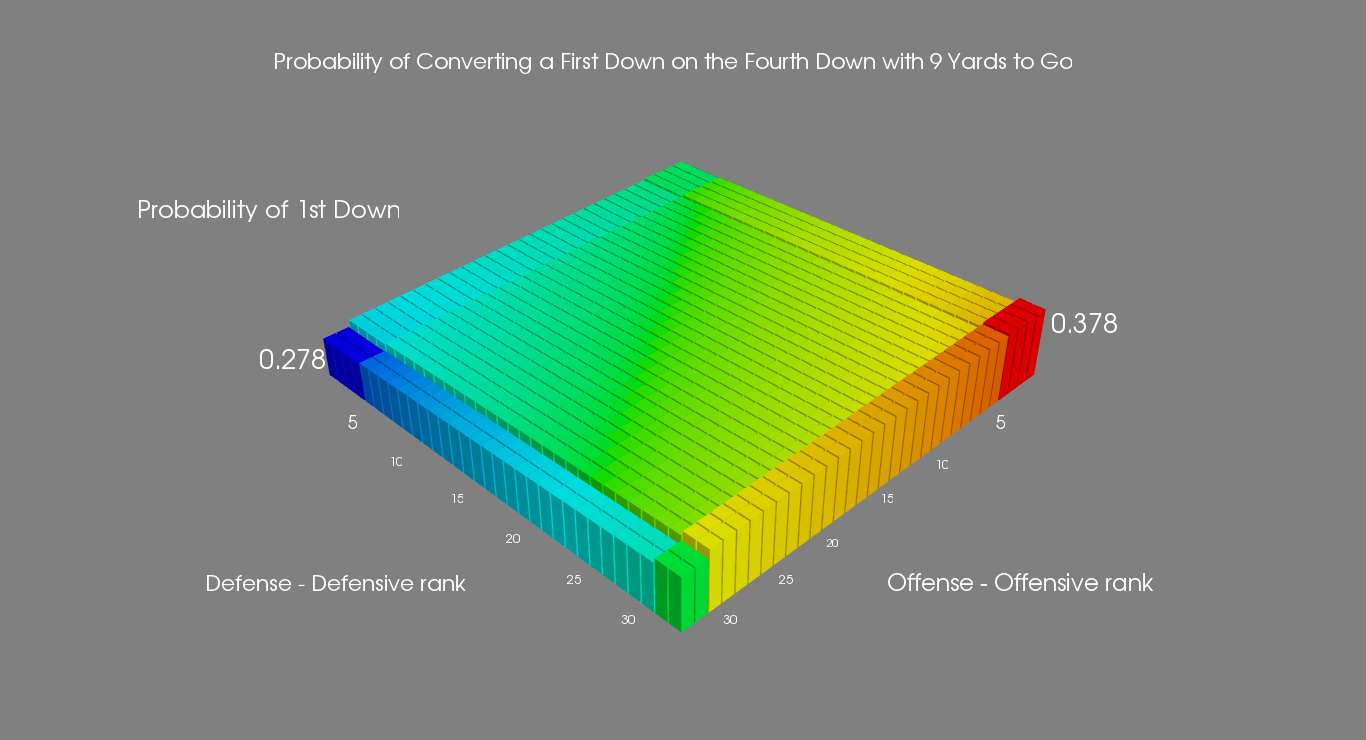
\includegraphics[width=1\textwidth]{ProbConv9.png}
\end{center}
\end{figure}
  \end{frame}
  \begin{frame}
    \frametitle{\centerline{NFL Go For It!}}
\begin{figure}
\begin{center}
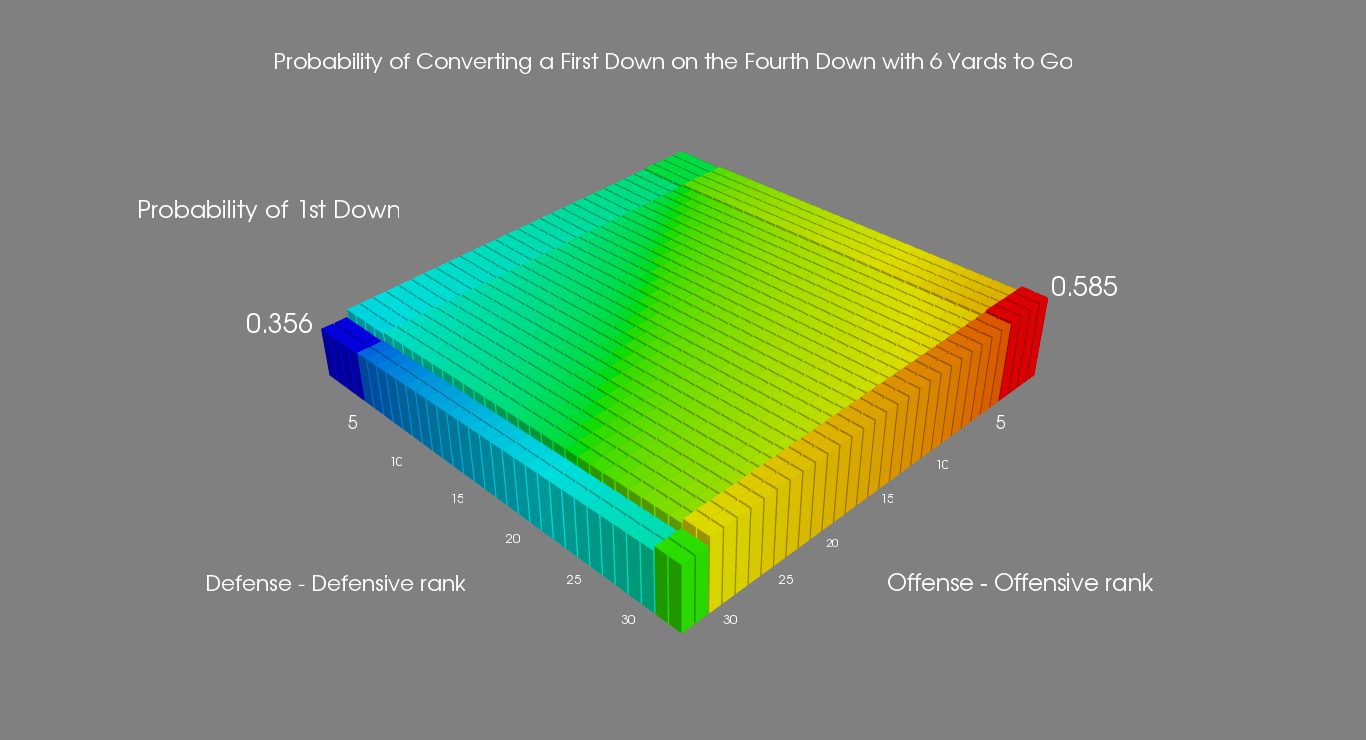
\includegraphics[width=1\textwidth]{ProbConv6.png}
\end{center}
\end{figure}
  \end{frame}
  \begin{frame}
    \frametitle{\centerline{NFL Go For It!}}
\begin{figure}
\begin{center}
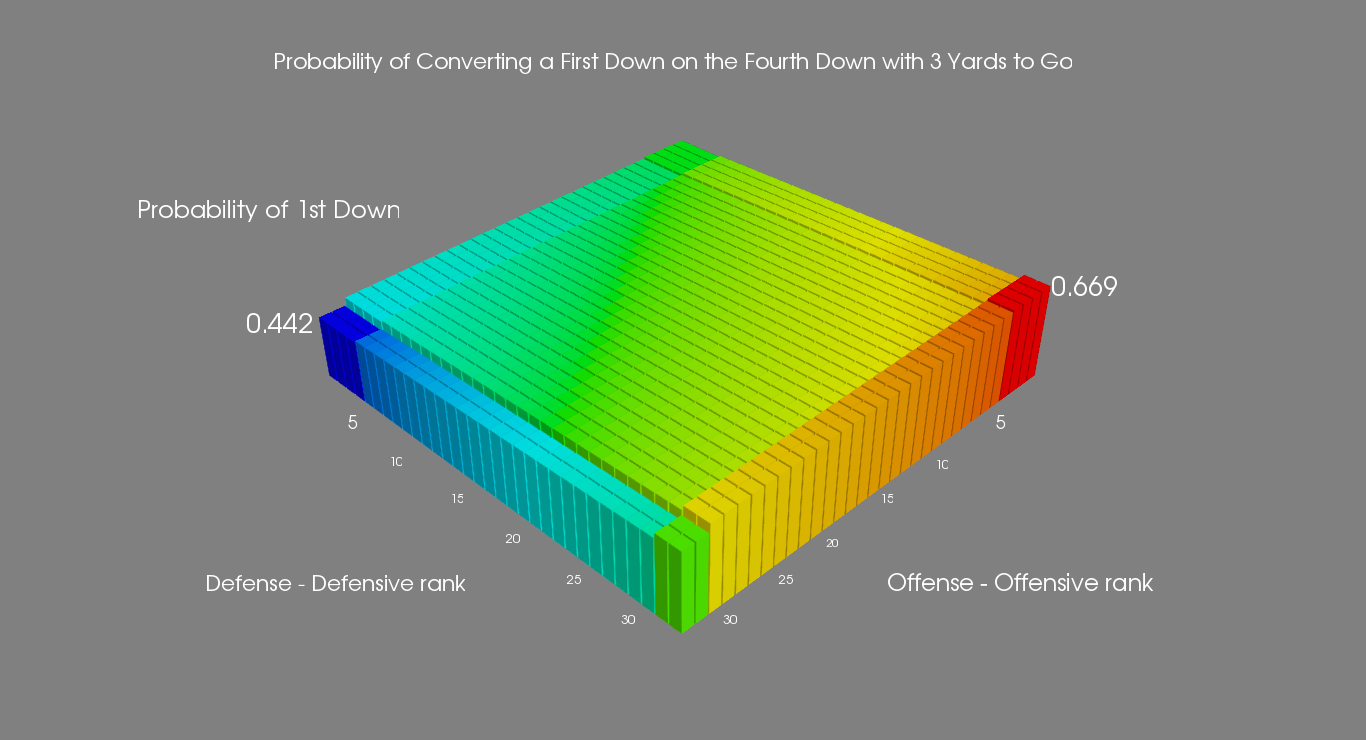
\includegraphics[width=1\textwidth]{ProbConv3.png}
\end{center}
\end{figure}
  \end{frame}
  \begin{frame}
    \frametitle{\centerline{NFL Go For It!}}
\begin{figure}
\begin{center}
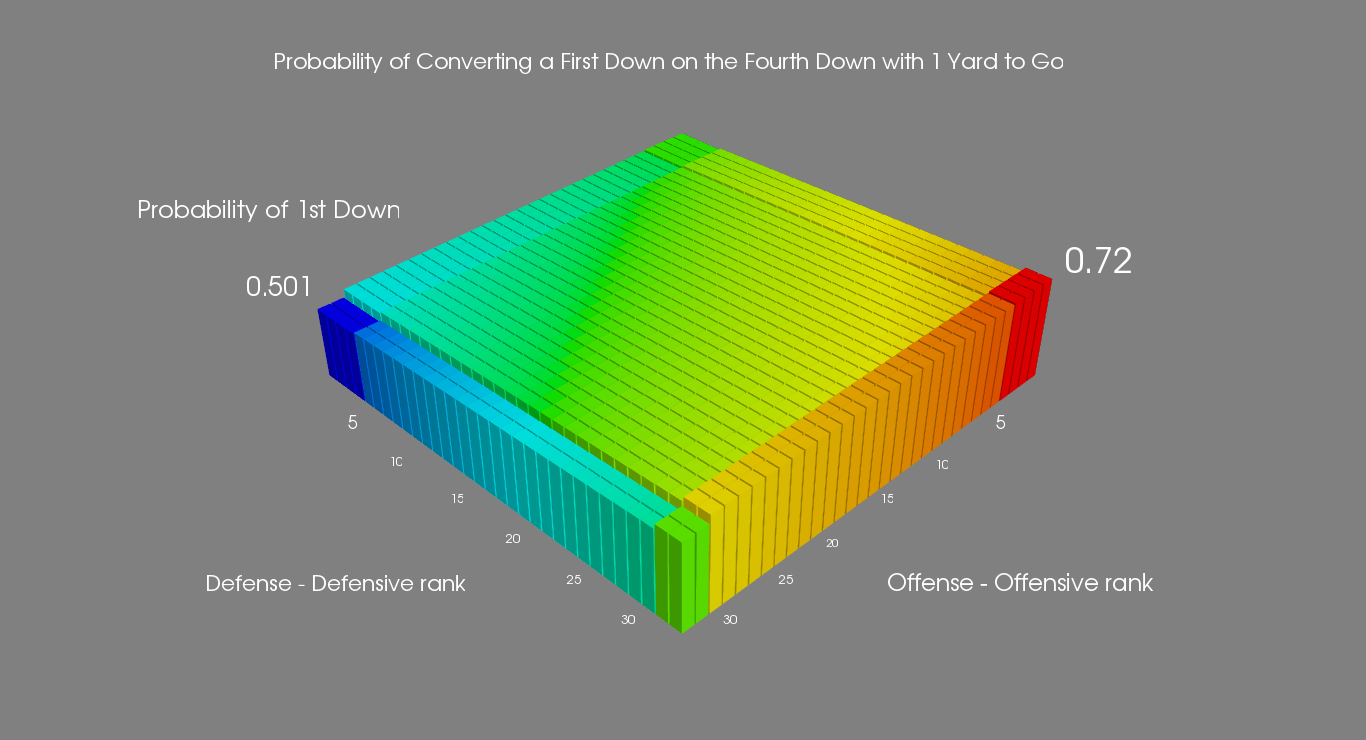
\includegraphics[width=1\textwidth]{ProbConv1.png}
\end{center}
\end{figure}
  \end{frame}
  \begin{frame}
    \frametitle{\centerline{NFL Go For It!}}
\begin{figure}
\begin{center}
Offense Ranking: Offensive 1, Defensive 1\\
Defense Ranking: Offensive 25, Defensive 25
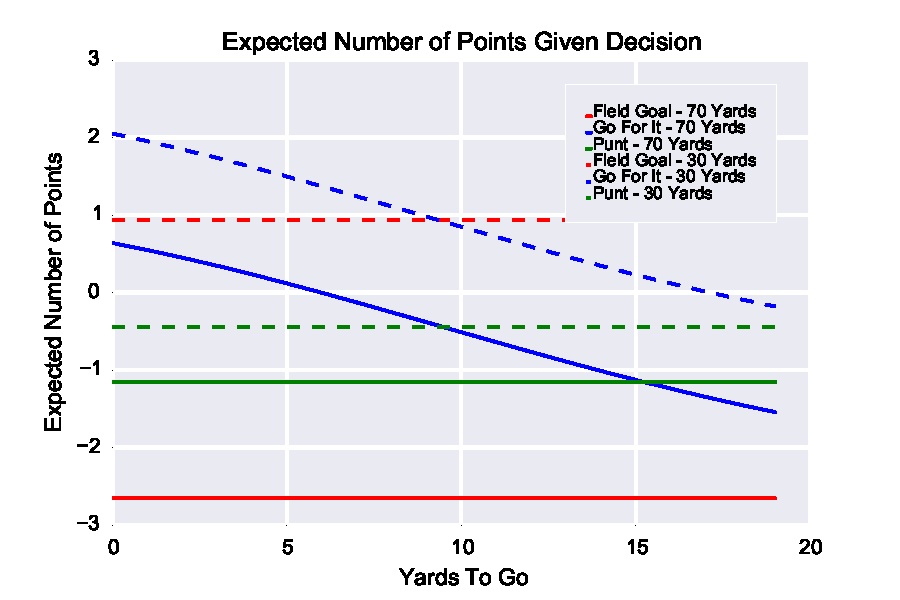
\includegraphics[width=1\textwidth]{Decision3070112525.pdf}
\end{center}
\end{figure}
  \end{frame}
  \begin{frame}
    \frametitle{\centerline{NFL Go For It!}}
\begin{figure}
\begin{center}
Offense Ranking: Offensive 25, Defensive 25\\
Defense Ranking: Offensive 1, Defensive 1
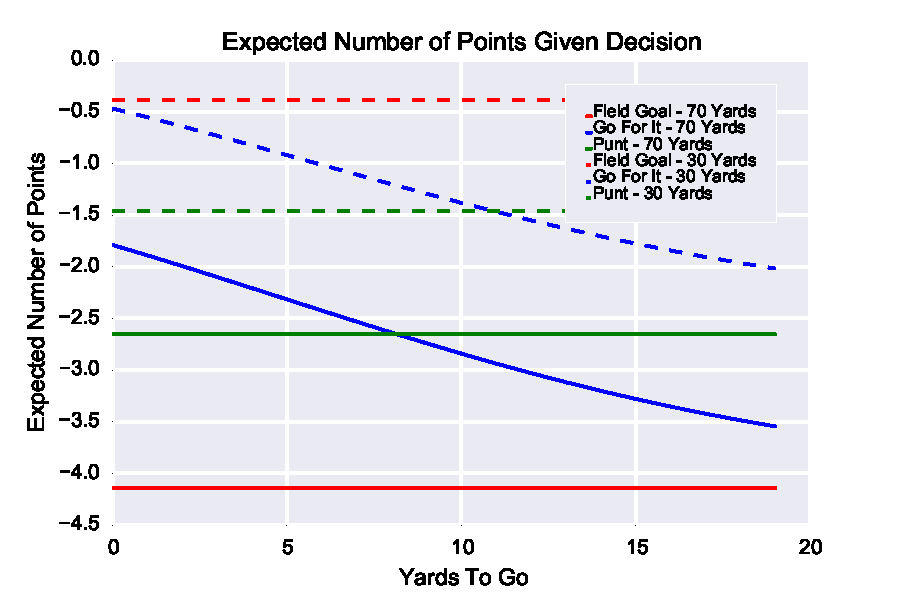
\includegraphics[width=1\textwidth]{Decision3070252511.pdf}
\end{center}
\end{figure}
  \end{frame}
 \begin{frame}
    \frametitle{\centerline{NFL Go For It!}\\ \centerline{What should my decision be?}}
\begin{center}
Offense Ranking: Offensive 1, Defensive 1\\
Defense Ranking: Offensive 25, Defensive 25
\end{center}
\begin{figure}
\begin{center}
Yard Line
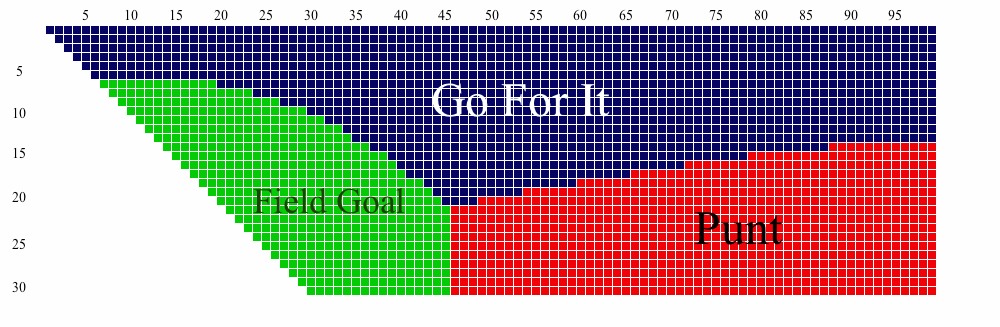
\includegraphics[width=1\textwidth]{GridBlock112525.png}
\end{center}
\end{figure}
  \end{frame}
\begin{frame}
    \frametitle{\centerline{NFL Go For It!}\\ \centerline{What should my decision be?}}
\begin{center}
Offense Ranking: Offensive 15, Defensive 15\\
Defense Ranking: Offensive 15, Defensive 15
\end{center}
\begin{figure}
\begin{center}
Yard Line
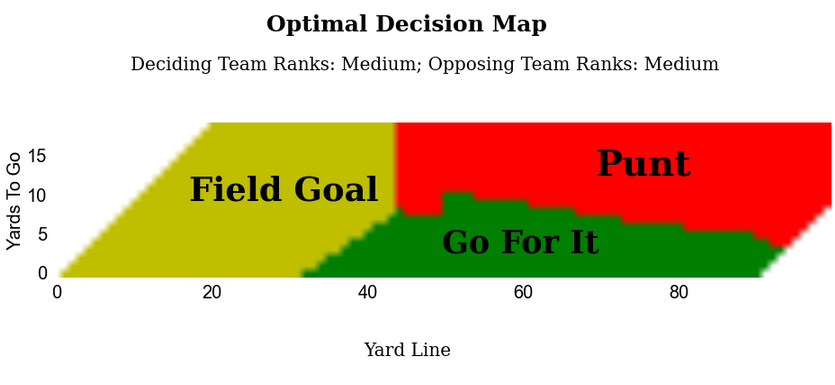
\includegraphics[width=1\textwidth]{GridBlock15151515.png}
\end{center}
\end{figure}
  \end{frame}
\begin{frame}
    \frametitle{\centerline{NFL Go For It!}\\ \centerline{What should my decision be?}}
\begin{center}
Offense Ranking: Offensive 25, Defensive 25\\
Defense Ranking: Offensive 2, Defensive 2
\end{center}
\begin{figure}
\begin{center}
Yard Line
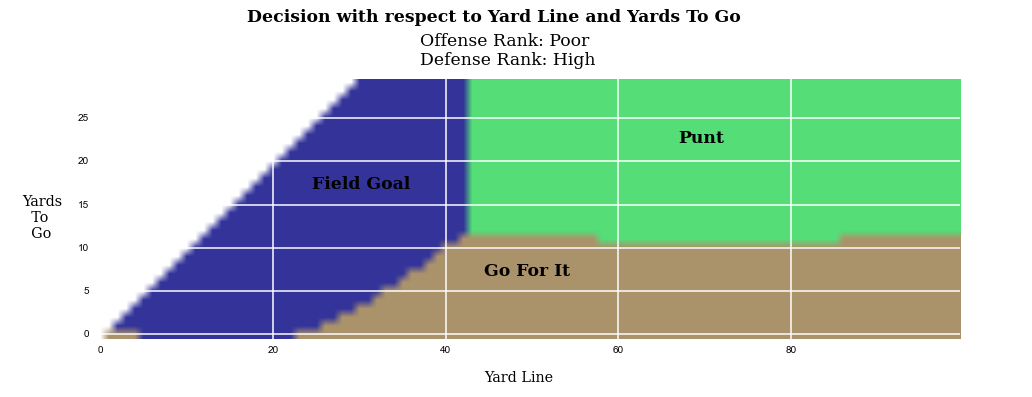
\includegraphics[width=1\textwidth]{GridBlock252522.png}
\end{center}
\end{figure}
  \end{frame}
\end{document}